\documentclass[conference]{IEEEtran}
\usepackage{cite}
\usepackage{amsmath}
\usepackage{newtxtext,newtxmath}
\usepackage{graphicx}
\usepackage{booktabs}
\usepackage{multirow}
\usepackage{array}
\usepackage{tabularx}
\usepackage{xcolor}
\usepackage[hidelinks]{hyperref}

\newcommand{\spmu}{speech+music}
\newcolumntype{Y}{>{\raggedright\arraybackslash}X}

\begin{document}

\title{Right but Unsure: How Focal Loss and Label Smoothing Miscalibrate Multi-Class Voice Activity Detection}

\maketitle

\begin{abstract}
Voice activity detectors (VADs) output confidence scores that deployed systems act on through fixed thresholds, so the scores must be calibrated. Multi-class detectors, which separate speech, music and overlapping speech and music, face strong class imbalance, and class weighting, focal loss and label smoothing are common remedies. We measure what these remedies do to calibration. A compact convolutional recurrent network is trained on labelled mixtures of public corpora with four losses, three seeds each, and evaluated on in-domain audio and on audio from unseen source corpora. Plain cross-entropy is well calibrated, with an expected calibration error (ECE) of 0.010. Focal loss and label smoothing raise it to 0.105 and 0.059 and make the detector under-confident, without improving macro-F1 or the F1 score of the rare overlapping class. As a result, fixed thresholds change meaning: at a confidence threshold of 0.9 the cross-entropy model accepts 81\% of frames, the label-smoothing model 59\% and the focal-loss model 35\%. A single temperature fitted on validation data restores calibration for focal loss on both test sets (ECE 0.112 to 0.006 on unseen sources) and largely for label smoothing. We conclude that for compact VADs these losses cost calibration without buying accuracy, and that any change of training loss should be followed by recalibration.
\end{abstract}

\begin{IEEEkeywords}
voice activity detection, confidence calibration, focal loss, label smoothing, temperature scaling, class imbalance
\end{IEEEkeywords}

% =====================================================================
\section{Introduction}

Voice activity detection (VAD) decides, frame by frame, whether speech is present, and gates more expensive processing such as speech recognition, speaker diarization and dialogue enhancement. Recent work pushes VADs towards very small, low-latency models for always-on devices~\cite{bauer2026kilovad,cohen2026s4vad,jafarzadeh2025tinyvad}. In deployment, the detector's output is rarely used as a hard label: a system wakes up, transmits or enhances audio when a score exceeds a threshold. Such thresholds are only meaningful if the scores are \emph{calibrated}, that is, if frames scored 0.9 are correct about 90\% of the time~\cite{guo2017calibration}.

Many applications need more than speech versus non-speech. Broadcast monitoring, music-aware speech recognition and dialogue enhancement must tell speech from music and must detect speech that overlaps with music~\cite{grundhuber2025srsad,hung2021avaspeechsmad}. A multi-class VAD with the classes \emph{background}, \emph{speech}, \emph{music} and \emph{\spmu} faces a strong imbalance: overlapping speech and music is rare in natural audio. The usual remedies are class-weighted cross-entropy, focal loss~\cite{lin2017focal} and label smoothing~\cite{muller2019labelsmoothing}. The latter two are also promoted as ways to \emph{improve} calibration, because they counteract the over-confidence of large networks~\cite{mukhoti2020focal,muller2019labelsmoothing}.

Two questions have not been answered for this setting. First, recent VAD studies report AUC, F1 or latency but do not examine whether their scores are calibrated (Section~\ref{sec:related}). Second, calibration studies in speech and audio target recognition, captioning and bioacoustics~\cite{huo2025overconfidence,dunker2025aac,schwinger2026bird}, not frame-level multi-class VAD, and it is unknown what imbalance-oriented losses do to the confidence of a compact detector.

This paper answers both questions in a controlled study. Its contributions are:
\begin{enumerate}
\item To our knowledge, the first calibration study of a four-class VAD, using synthetic mixtures with exact frame labels and clip-level bootstrap intervals.
\item Evidence that focal loss and label smoothing make a compact detector strongly \emph{under}-confident while giving no accuracy benefit, including for the rare class; the effect is significant in every seed.
\item A demonstration that this changes what a fixed confidence threshold means, and that one fitted temperature restores it on in-domain audio and on audio from unseen source corpora.
\end{enumerate}

% =====================================================================
\section{Related Work}\label{sec:related}

\textbf{Voice activity detection.} Recent VAD research concentrates on accuracy, robustness and efficiency. kiloVAD~\cite{bauer2026kilovad} reaches 0.850 AUC on AVA-Speech with about 2\,k parameters; S4VAD~\cite{cohen2026s4vad} uses state-space models and a latency-aware evaluation; SincQDR-VAD~\cite{wang2025sincqdr} trains with a ranking loss that optimises AUROC; FusionVAD~\cite{tripathi2025fusionvad} fuses MFCCs with pretrained speech features; and further work targets noise robustness~\cite{jafarzadeh2025tinyvad,bovbjerg2025tsvad}. Beyond binary detection, foreground VAD~\cite{yang2026fvad} and personal VAD~\cite{ding2020personalvad,yeh2025pvad} separate target from background speakers, overlapped-speech detection~\cite{sun2025osd} separates one from several talkers, and SR-SAD~\cite{grundhuber2025srsad} rejects singing. As Table~\ref{tab:related} shows, none of these studies measures whether the output scores are calibrated, and the only one that compares losses for imbalance~\cite{yeh2025pvad} evaluates them by accuracy alone.

\textbf{Calibration in speech and audio.} Over-confidence of modern networks and its correction by temperature scaling were established by Guo et al.~\cite{guo2017calibration}; classwise calibration error was introduced by Kull et al.~\cite{kull2019dirichlet}. Recent work analyses the theory of temperature scaling~\cite{mattei2026welltempered}, benchmarks post-hoc calibrators on tabular and vision data~\cite{berta2026calarena}, and studies calibration under label noise and domain shift~\cite{penso2026thesis}. In audio, Whisper is over-confident in noise~\cite{huo2025overconfidence}, captioning models are over-confident regardless of semantic accuracy~\cite{dunker2025aac}, and multi-label bird-sound classifiers can be under-confident~\cite{schwinger2026bird}. None of these covers VAD.

\textbf{Losses and calibration.} Focal loss~\cite{lin2017focal} and label smoothing~\cite{muller2019labelsmoothing} reduce over-confidence in image classification~\cite{mukhoti2020focal}. AdaFocal~\cite{ghosh2022adafocal} showed that a fixed focal parameter can leave samples under-confident, and recent work notes that label smoothing only addresses over-confidence~\cite{bahavan2026fedlas} and that focal-type weighting does not align with sample uncertainty~\cite{lin2025uwg}. Confidence-aware reweighting for long-tailed data~\cite{jagati2026ccar} targets accuracy and does not evaluate calibration. These studies mostly concern large vision networks, whose cross-entropy baselines are typically over-confident~\cite{guo2017calibration}.

\textbf{Research gap.} No prior work measures the calibration of a multi-class VAD, and the effect of imbalance-oriented losses on the confidence of a compact audio detector, whose baseline need not be over-confident, has not been studied. Nor has the consequence for fixed operating thresholds been quantified.

\begin{table*}[t]
\caption{Recent related work (2025--2026) and the gap each leaves for this study.}
\label{tab:related}
\centering
\footnotesize
\setlength{\tabcolsep}{4pt}
\begin{tabularx}{\textwidth}{@{}p{2.75cm}p{5.6cm}cY@{}}
\toprule
\textbf{Work} & \textbf{Task and classes} & \textbf{Calib.} & \textbf{Gap relative to this work} \\
\midrule
kiloVAD~\cite{bauer2026kilovad} & Ultra-tiny causal VAD, speech vs.\ non-speech & no & Binary; reports AUC, never checks whether scores are calibrated \\
S4VAD~\cite{cohen2026s4vad} & State-space VAD, onset-latency evaluation & no & Binary; latency metric, frame-score calibration unexamined \\
Foreground VAD~\cite{yang2026fvad} & Dominant speaker vs.\ background talkers & no & No music classes; no confidence analysis \\
SR-SAD~\cite{grundhuber2025srsad} & Speech activity robust to singing voice & no & Speech vs.\ singing only; AUC only, no loss comparison \\
FusionVAD~\cite{tripathi2025fusionvad} & Binary VAD, MFCC + pretrained features & no & Accuracy and efficiency only; no calibration or loss study \\
SincQDR-VAD~\cite{wang2025sincqdr} & Binary VAD, ranking loss for AUROC & no & Optimises ranking, explicitly not probabilities \\
TS-VAD~\cite{bovbjerg2025tsvad} & Target-speaker VAD in noise, SSL pre-training & no & Robustness only; confidence not assessed \\
Tiny VAD~\cite{jafarzadeh2025tinyvad} & Binary VAD for voice assistants in noise & no & Accuracy in noise only \\
WavLM OSD~\cite{sun2025osd} & Overlapping-speech detection & no & Speaker overlap, not speech/music; F1 only \\
PVAD study~\cite{yeh2025pvad} & Personal VAD, losses for imbalance & no & Imbalance losses judged by accuracy, not calibration \\
\midrule
Noisy ASR~\cite{huo2025overconfidence} & Token confidence of Whisper in noise & yes & ASR over-confidence; not frame-level detection \\
Captioning~\cite{dunker2025aac} & Confidence of audio captioning models & yes & Sequence generation; no loss-induced under-confidence \\
Bird sound~\cite{schwinger2026bird} & Multi-label bioacoustic classification & yes & Notes under-confidence but does not link it to the loss \\
CalArena~\cite{berta2026calarena} & Post-hoc calibrator benchmark & yes & Tabular and vision only; no training losses \\
Well-tempered~\cite{mattei2026welltempered} & Theory of temperature scaling & yes & Theoretical; no audio, no training-loss effects \\
CCAR~\cite{jagati2026ccar} & Confidence-aware reweighting, long-tailed images & partly & Targets accuracy; calibration not evaluated \\
FedLAS~\cite{bahavan2026fedlas} & Bidirectional label smoothing, images & yes & Vision only; no detection or audio \\
UWG~\cite{lin2025uwg} & Focal-loss family analysis, images & yes & Vision only; no fixed-threshold consequence \\
\bottomrule
\end{tabularx}
\end{table*}

% =====================================================================
\section{Method}\label{sec:method}

\begin{figure*}[t]
\centering
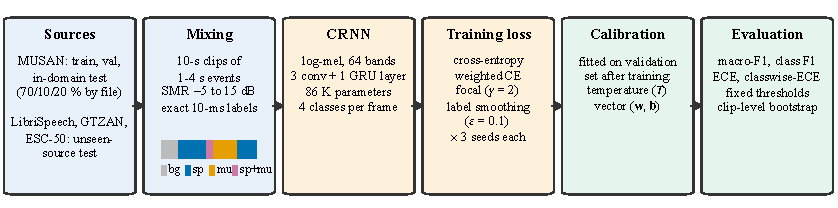
\includegraphics[width=\textwidth]{figures/fig1_method.pdf}
\caption{Study design. Labelled mixtures are generated from public corpora, a compact CRNN is trained with four losses (three seeds each), calibrators are fitted on validation data, and calibration, accuracy and threshold behaviour are evaluated on an in-domain test set and on a test set built from unseen source corpora. The colour strip illustrates the frame labels of one clip.}
\label{fig:method}
\end{figure*}

\subsection{Task and data}
Each 10-ms frame is assigned one of four classes: background (silence or noise), speech (with or without noise), music (singing counts as music) and \spmu. Fig.~\ref{fig:method} summarises the design. Exact labels are essential for measuring calibration, so the data are synthetic mixtures with known ground truth. MUSAN~\cite{snyder2015musan} speech, music and noise files are split by file into training (70\%), validation (10\%) and in-domain test (20\%) pools. An \emph{unseen-source} test set uses LibriSpeech test-clean~\cite{panayotov2015librispeech} speech, GTZAN~\cite{tzanetakis2002genre} music without the hip-hop genre (rap is speech-like) and ESC-50~\cite{piczak2015esc} noise without its human-vocal classes.

Each 10-s clip at 16\,kHz consists of a quiet noise bed and a sequence of 1--4\,s events whose class is drawn with probabilities 0.25/0.50/0.20/0.05 (background/speech/music/\spmu). Speech-over-music events use a speech-to-music ratio of $-5$, 0, 5, 10 or 15\,dB. Speech labels come from an energy detector on the clean speech (frames within 35\,dB of the segment peak, pauses under 150\,ms bridged), music labels from the placed music above $-60$\,dBFS. The splits contain 7{,}200 training clips (20\,h), 700 validation clips and 1{,}000 clips in each test set. The resulting frame shares are about 30\% background, 45\% speech, 21\% music and 4\% \spmu.

\subsection{Model and training}
The detector is a CRNN with 64-band log-mel input (25-ms window, 10-ms hop), three convolutional blocks (16, 32 and 64 channels, pooling over frequency only), one GRU layer with 64 units and a linear output of four logits per frame (85.6\,k parameters). It is trained with Adam (learning rate $10^{-3}$, batch 32, random 4-s crops) for up to 20 epochs, with early stopping on validation macro-F1. Four losses are compared: cross-entropy (CE); weighted CE with inverse-frequency class weights normalised to mean one; focal loss~\cite{lin2017focal} with $\gamma=2$; and label smoothing~\cite{muller2019labelsmoothing} with $\varepsilon=0.1$. Each loss is trained with three seeds, giving 12 models.

\subsection{Calibration measures and post-hoc calibration}
For $N$ test frames with predicted class $\hat{y}_i$ and confidence $\hat{p}_i=\max_k p_{ik}$, frames are grouped into $B=15$ equal-width confidence bins $S_b$ and
\begin{equation}
\mathrm{ECE}=\sum_{b=1}^{B}\frac{|S_b|}{N}\,\bigl|\mathrm{acc}(S_b)-\mathrm{conf}(S_b)\bigr| .
\end{equation}
Classwise-ECE~\cite{kull2019dirichlet} applies the same measure to each class probability and averages over classes. Frames within a clip are strongly correlated, so 95\% confidence intervals and paired comparisons use 1{,}000 bootstrap resamples of \emph{clips}, not frames.

Two calibrators are fitted on the validation set by minimising the negative log-likelihood: temperature scaling~\cite{guo2017calibration}, $\mathbf{p}=\mathrm{softmax}(\mathbf{z}/T)$, which never changes the predicted class; and vector scaling, $\mathbf{p}=\mathrm{softmax}(\mathbf{w}\odot\mathbf{z}+\mathbf{b})$ with one weight and bias per class. $T<1$ sharpens the scores and therefore indicates an under-confident model.

\subsection{Threshold behaviour}
To quantify what calibration means for a deployed system, we compute the \emph{coverage} $C(\tau)$, the share of frames whose confidence is at least a fixed threshold $\tau\in\{0.5,\dots,0.95\}$, together with the accuracy of those frames. For a calibrated model, the frames accepted at $\tau$ have an accuracy of at least $\tau$, and coverage is as high as accuracy allows.

% =====================================================================
\section{Results}\label{sec:results}

\begin{table*}[t]
\caption{Accuracy and calibration of the uncalibrated models (mean $\pm$ std over three seeds). Best value per column in bold. sp+mu: speech+music class.}
\label{tab:main}
\centering
\footnotesize
\setlength{\tabcolsep}{4.5pt}
\begin{tabular}{@{}lcccc|cccc@{}}
\toprule
& \multicolumn{4}{c|}{\textbf{In-domain test}} & \multicolumn{4}{c}{\textbf{Unseen-source test}} \\
\textbf{Loss} & Macro-F1\,$\uparrow$ & F1 sp+mu\,$\uparrow$ & ECE\,$\downarrow$ & cw-ECE\,$\downarrow$ & Macro-F1\,$\uparrow$ & F1 sp+mu\,$\uparrow$ & ECE\,$\downarrow$ & cw-ECE\,$\downarrow$ \\
\midrule
Cross-entropy & \textbf{0.875}\,$\pm$\,.003 & \textbf{0.710}\,$\pm$\,.018 & \textbf{0.010}\,$\pm$\,.003 & \textbf{0.009}\,$\pm$\,.003 & \textbf{0.878}\,$\pm$\,.011 & \textbf{0.740}\,$\pm$\,.022 & 0.010\,$\pm$\,.005 & \textbf{0.011}\,$\pm$\,.006 \\
Weighted CE & 0.862\,$\pm$\,.008 & 0.680\,$\pm$\,.023 & 0.011\,$\pm$\,.004 & 0.015\,$\pm$\,.001 & 0.863\,$\pm$\,.005 & 0.701\,$\pm$\,.013 & \textbf{0.009}\,$\pm$\,.005 & 0.022\,$\pm$\,.002 \\
Focal loss & 0.865\,$\pm$\,.003 & 0.686\,$\pm$\,.007 & 0.105\,$\pm$\,.008 & 0.054\,$\pm$\,.005 & 0.873\,$\pm$\,.004 & 0.730\,$\pm$\,.009 & 0.112\,$\pm$\,.009 & 0.058\,$\pm$\,.005 \\
Label smoothing & 0.866\,$\pm$\,.003 & 0.688\,$\pm$\,.011 & 0.059\,$\pm$\,.007 & 0.035\,$\pm$\,.001 & 0.874\,$\pm$\,.008 & 0.736\,$\pm$\,.005 & 0.060\,$\pm$\,.012 & 0.037\,$\pm$\,.000 \\
\bottomrule
\end{tabular}
\end{table*}

\subsection{Accuracy is similar, calibration is not}
Table~\ref{tab:main} shows that all four losses reach a similar accuracy, with plain CE the most accurate: macro-F1 0.875 in-domain against 0.862--0.866 for the alternatives. None of the imbalance-oriented losses improves the rare \spmu{} class, whose F1 is 0.710 with CE and 0.680--0.688 otherwise. Calibration, in contrast, differs by an order of magnitude. CE has an ECE of 0.010 and weighted CE of 0.011, whereas focal loss reaches 0.105 and label smoothing 0.059. The paired clip bootstrap confirms that the ECE increase of focal loss and label smoothing over CE is significant in all three seeds on both test sets. Weighted CE leaves the top-label ECE unchanged but nearly doubles the classwise-ECE (0.015 against 0.009 in-domain).

\begin{figure}[t]
\centering
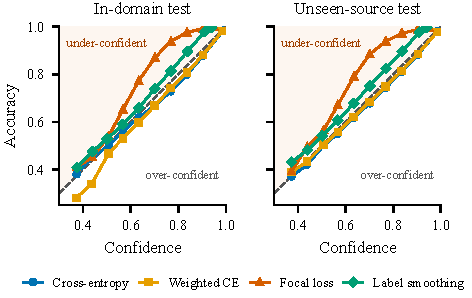
\includegraphics[width=\columnwidth]{figures/fig2_reliability.pdf}
\caption{Reliability diagrams of the uncalibrated models (bins pooled over three seeds; bins with fewer than 0.1\% of frames omitted). Points above the diagonal are under-confident: the model is right more often than it claims.}
\label{fig:reliability}
\end{figure}

\subsection{The miscalibration is under-confidence}
The reliability diagrams in Fig.~\ref{fig:reliability} show the direction. CE and weighted CE lie close to the diagonal, with a mild over-confidence of 3--4 points in the 0.7--0.9 confidence range, which contains about 18\% of the frames. Focal loss and label smoothing lie clearly \emph{above} the diagonal: in the bin around 0.7 confidence, focal-loss frames are correct about 87\% of the time. The fitted temperatures agree. They are $1.06\pm0.04$ for CE and $1.07\pm0.06$ for weighted CE, so these models are very slightly over-confident, but $0.53\pm0.02$ for focal loss and $0.68\pm0.02$ for label smoothing, which means their scores must be sharpened, not softened.

\begin{figure}[t]
\centering
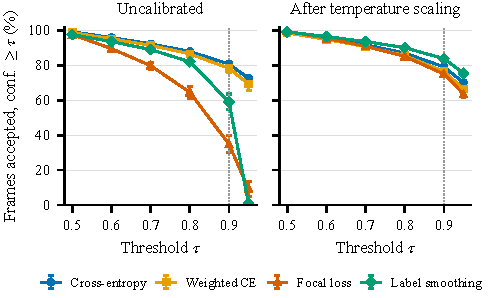
\includegraphics[width=\columnwidth]{figures/fig3_coverage.pdf}
\caption{Share of in-domain frames accepted at a fixed confidence threshold $\tau$ (mean $\pm$ std over seeds), before and after temperature scaling. The dotted line marks $\tau=0.9$.}
\label{fig:coverage}
\end{figure}

\subsection{Fixed thresholds change meaning}
Fig.~\ref{fig:coverage} shows the practical consequence. At $\tau=0.9$, the CE model accepts 80.6\% of in-domain frames, weighted CE 78.3\%, label smoothing 59.1\% and focal loss only 34.9\%, although all four models are about equally accurate. The accepted frames of the focal-loss model are correct 99.7\% of the time while their mean confidence is 93.5\%, so the threshold rejects many frames that the model in fact classifies correctly. The same pattern holds on the unseen-source test set (79.3\%, 76.4\%, 55.5\% and 30.4\%). After temperature scaling the curves nearly coincide: at $\tau=0.9$ the spread between losses shrinks from 46 to 9 percentage points (CE 79.0\%, weighted CE 76.5\%, focal 74.9\%, label smoothing 83.7\%). At the default threshold of 0.5, by contrast, all losses behave alike: false alarms of a speech-versus-rest decision are 4.6--4.9\% and misses 5.8--6.9\% in-domain, and calibration hardly changes them. The effect therefore matters exactly where high thresholds are used to suppress false triggers.

\begin{table}[t]
\caption{Fitted temperature and ECE before (raw) and after temperature (TS) and vector scaling (VS), means over three seeds.}
\label{tab:calib}
\centering
\footnotesize
\setlength{\tabcolsep}{3.2pt}
\begin{tabular}{@{}lc|ccc|ccc@{}}
\toprule
& & \multicolumn{3}{c|}{\textbf{In-domain}} & \multicolumn{3}{c}{\textbf{Unseen sources}} \\
\textbf{Loss} & $T$ & raw & TS & VS & raw & TS & VS \\
\midrule
Cross-entropy & 1.06 & 0.010 & 0.005 & 0.006 & 0.010 & 0.005 & 0.004 \\
Weighted CE & 1.07 & 0.011 & 0.006 & 0.007 & 0.009 & 0.003 & 0.003 \\
Focal loss & 0.53 & 0.105 & 0.007 & 0.005 & 0.112 & 0.006 & 0.006 \\
Label smoothing & 0.68 & 0.059 & 0.016 & 0.015 & 0.060 & 0.016 & 0.015 \\
\bottomrule
\end{tabular}
\end{table}

\begin{figure}[t]
\centering
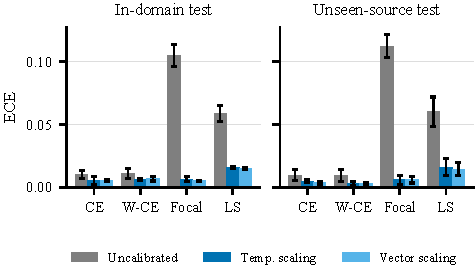
\includegraphics[width=\columnwidth]{figures/fig4_ece.pdf}
\caption{ECE before and after post-hoc calibration fitted on in-domain validation data (mean $\pm$ std over seeds). W-CE: weighted CE; LS: label smoothing.}
\label{fig:ece}
\end{figure}

\subsection{One temperature repairs the damage}
Table~\ref{tab:calib} and Fig.~\ref{fig:ece} show that a single temperature, fitted on in-domain validation data, removes most of the miscalibration. Focal-loss ECE falls from 0.105 to 0.007 in-domain and from 0.112 to 0.006 on unseen sources; label smoothing falls from about 0.060 to 0.016 on both sets; CE halves from 0.010 to 0.005. Temperature scaling reduced ECE significantly in 11 of 12 models in-domain and 10 of 12 on unseen sources, without changing any prediction. Vector scaling gives similar ECE and additionally recovers part of the accuracy lost by weighted CE on unseen sources: macro-F1 rises from 0.863 to 0.879 and \spmu{} F1 from 0.701 to 0.740.

\subsection{Robustness checks}
Two further analyses support these findings. First, the calibrators transfer to the unseen-source test set: accuracy and ECE there match the in-domain values (macro-F1 0.878 against 0.875 and ECE 0.010 for CE), so the calibration differences are not specific to the MUSAN recordings. Second, deployed VADs smooth their posteriors over time. A median filter of 5--21 frames raises CE macro-F1 by up to 0.004 (0.875 to 0.878 in-domain) and changes ECE by less than 0.001, both before and after temperature scaling. Smoothing therefore neither hides nor causes the miscalibration.

% =====================================================================
\section{Discussion}\label{sec:discussion}

\textbf{Why the losses backfire.} Focal loss and label smoothing were designed to counter the over-confidence of large networks~\cite{mukhoti2020focal,muller2019labelsmoothing}. A compact VAD trained with CE is already nearly calibrated ($T\approx1.06$), so the same corrections overshoot into under-confidence. This is consistent with the observation that a fixed focal parameter can leave samples under-confident~\cite{ghosh2022adafocal}. Label smoothing has a further, structural effect: with $\varepsilon=0.1$ and $K=4$ classes the training target for the correct class is $1-\varepsilon+\varepsilon/K=0.925$, so confidence rarely exceeds 0.95. This explains why the label-smoothing model accepts only 0.9\% of frames at $\tau=0.95$, and why we use $\tau=0.9$ for the main comparison.

\textbf{The rare class.} None of the imbalance-oriented losses improved \spmu{} detection. For weighted CE, the vector-scaling bias fitted for the \spmu{} class is strongly negative (about $-1.1$, against $-0.4$ for CE), which suggests that class weighting mainly shifts the decision towards the rare class rather than learning it better; correcting this shift after training recovered part of the lost accuracy.

\textbf{Practical recommendations.} For compact multi-class VADs we recommend (i) starting from plain cross-entropy, (ii) refitting a temperature on validation data whenever the training loss or its hyper-parameters change, and (iii) reporting calibration and coverage at the operating threshold alongside F1 or AUC.

\textbf{Scope.} The study uses one compact architecture and one setting per loss ($\gamma=2$, $\varepsilon=0.1$). The mixtures are synthetic, which gives exact frame labels but cleaner conditions than broadcast audio, and the unseen-source test changes the recordings while keeping the mixing recipe. As is standard practice~\cite{guo2017calibration}, the validation set serves both early stopping and calibrator fitting. Larger self-supervised models, sweeps over $\gamma$ and $\varepsilon$, and real recordings with co-occurrence labels~\cite{hung2021avaspeechsmad} are natural next steps.

% =====================================================================
\section{Conclusion}
We measured the calibration of a compact four-class voice activity detector trained with four losses. Plain cross-entropy produced the most accurate and best-calibrated detector. Focal loss and label smoothing, often used against class imbalance and over-confidence, made the detector strongly under-confident without improving the rare speech+music class, so that a threshold of 0.9 accepted between 35\% and 81\% of frames depending only on the loss. A single temperature fitted after training restored calibration on in-domain audio and on audio from unseen corpora. Calibration should therefore be reported, and re-established, whenever a VAD's training loss changes. Code and result tables will be released with the final version of the paper.

\bibliographystyle{IEEEtran}
\bibliography{refs}

\end{document}
